\documentclass{article}

\usepackage[utf8]{inputenc}
\usepackage[T1]{fontenc}
\usepackage[a4paper,margin=1in]{geometry}
\usepackage{amsmath}
\usepackage{booktabs}
\usepackage{natbib}
\usepackage{hyperref}
\usepackage{tabularx}
\usepackage{array}
\usepackage{pgfplots}
\usepackage{tikz}
\usepackage{xcolor}
\usepackage{siunitx}
\usepackage{cleveref}

\pgfplotsset{
    compat=1.18,
    my_style/.style={
        width=0.9\textwidth,
        axis lines=left,
        grid=major,
        grid style={dashed, gray!50},
        legend style={draw=none, fill=none, at={(0.5,-0.2)}, anchor=north}
    }
}

\title{Comparative Analysis of NVIDIA and AMD in the Data Center GPU Market (2022--2024)}
\author{Research Synthesis Team}
\date{June 2024}

\begin{document}

\maketitle

\begin{abstract}
This report presents a comprehensive comparative analysis of NVIDIA and AMD in the data center GPU market from 2022 to 2024. Leveraging financial data, market share statistics, shipment volumes, and key performance drivers, we examine the explosive growth of the sector, NVIDIA's continued dominance, and AMD's rapid expansion. The analysis integrates quantitative trends, technological innovations, and strategic partnerships, providing insights into the evolving competitive landscape and future outlook for data center GPUs.
\end{abstract}

\section{Introduction}

The data center GPU market has emerged as a critical arena for semiconductor companies, propelled by the rapid proliferation of artificial intelligence (AI), machine learning (ML), and high-performance computing (HPC) workloads. GPUs are indispensable for accelerating AI model training and inference, fueling unprecedented demand from cloud service providers, enterprises, and hyperscalers. NVIDIA and AMD are the primary competitors, with NVIDIA historically leading due to early investments in AI-optimized architectures and a robust software ecosystem.

Between 2022 and 2024, the market experienced explosive growth, driven by generative AI applications and cloud-based AI services. NVIDIA's data center GPU revenue more than quadrupled, while AMD's segment nearly doubled, reflecting both companies' strategic focus on AI workloads. This report synthesizes financial data, market share statistics, growth trends, and performance drivers to provide a detailed comparative analysis of NVIDIA and AMD's data center GPU businesses.

\section{Financial Performance and Revenue Trends}

\subsection{Annual and Quarterly Revenue Comparison}

\begin{table}[ht]
\centering
\caption{Data Center Revenue and Growth (2022--2024)}
\label{tab:revenue}
\begin{tabularx}{\textwidth}{l
    S[table-format=2.2]
    S[table-format=2.2]
    l
    l
}
\toprule
Year & {NVIDIA Data Center Revenue (B USD)} & {AMD Data Center Revenue (B USD)} & NVIDIA YoY Growth & AMD YoY Growth \\
\midrule
2022   & 11.7  & 6.5   & -      & -     \\
2023   & 27.0  & 6.6   & 130\%  & 3\%   \\
2024   & 47.5  & 12.6  & 76\%   & 94\%  \\
Q1 2024 & 4.28 & 1.2   & 61\%   & 20\%  \\
Q4 2024 & 18.4 & 3.9   & 409\%  & 69\%  \\
\bottomrule
\end{tabularx}
\end{table}

NVIDIA's data center revenue surged from approximately \$11.7 billion in 2022 to \$47.5 billion in 2024, driven by AI demand and new GPU architectures \cite{nvidia2024results, fiscalai}. AMD's data center revenue nearly doubled from an estimated \$6.5 billion in 2022 to \$12.6 billion in 2024, fueled by growth in Instinct GPUs and EPYC CPUs \cite{amd2024results, constellation2024}. Quarterly data shows NVIDIA's Q4 2024 data center revenue at \$18.4 billion (409\% YoY increase), while AMD's Q4 2024 data center revenue was \$3.9 billion (69\% YoY increase) \cite{nvidia2024results, amd2024results}.

\begin{figure}[ht]
\centering
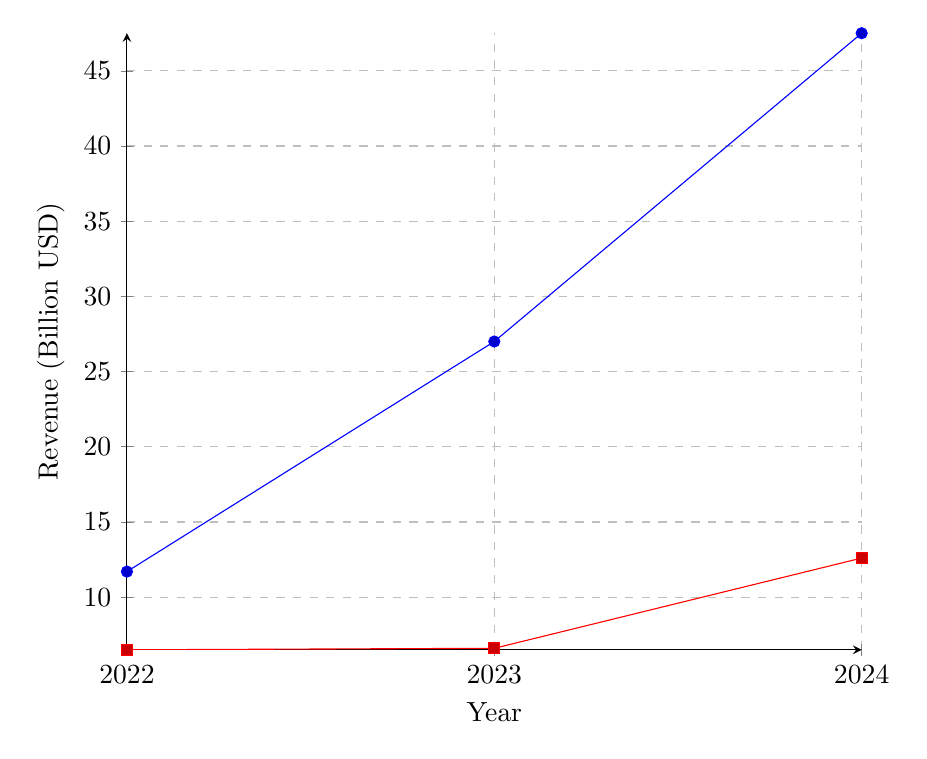
\begin{tikzpicture}
\begin{axis}[my_style, ylabel={Revenue (Billion USD)}, xlabel={Year}, xtick=data, symbolic x coords={2022,2023,2024}, legend columns=2, legend to name=legend1]
\addplot+[color=blue, mark=*] coordinates {(2022,11.7) (2023,27.0) (2024,47.5)};
\addplot+[color=red, mark=square*] coordinates {(2022,6.5) (2023,6.6) (2024,12.6)};
\legend{NVIDIA, AMD}
\end{axis}
\end{tikzpicture}
\caption{Annual Data Center Revenue: NVIDIA vs. AMD (2022--2024)}
\label{fig:revenue}
\end{figure}

\subsection{Growth Rates and Margins}

NVIDIA's data center GPU revenue grew at a compound annual growth rate (CAGR) of approximately 30\% from 2022 to 2024, while AMD's segment grew at a CAGR of about 15\% \cite{researchgate2024}. NVIDIA's gross margins improved significantly, reaching 76\% in Q4 2024, with net income surging 769\% year-over-year \cite{nvidia2024results}. AMD's gross margin for 2024 was approximately 49\% (GAAP), with operating income for the data center segment rising from \$1.3 billion in 2023 to \$3.5 billion in 2024 \cite{amd2024annual}.

\section{Market Share and Shipment Volumes}

\begin{table}[ht]
\centering
\caption{Market Share and Shipments (2022--2025)}
\label{tab:marketshare}
\begin{tabularx}{\textwidth}{l
    S[table-format=2.2]
    S[table-format=2.2]
    S[table-format=1.2]
    S[table-format=1.2]
    S[table-format=1.2]
}
\toprule
Year & {NVIDIA Market Share (\%)} & {AMD Market Share (\%)} & {Total Shipments (M Units)} & {NVIDIA Shipments (M)} & {AMD Shipments (M)} \\
\midrule
2022   & 98 & 2  & 2.67 & 2.64 & 0.03 \\
2023   & 98 & 2  & 3.85 & 3.76 & 0.50 \\
Q1 2025 & 90 & 10 & N/A  & N/A  & N/A  \\
\bottomrule
\end{tabularx}
\end{table}

NVIDIA shipped 3.76 million data center GPUs in 2023, maintaining a 98\% market share in shipments, up from 2.64 million in 2022 \cite{hpcwire2023, datacenterdynamics2023}. AMD shipped approximately 500,000 data center GPUs in 2023, increasing its presence but still holding a small market share (about 10\% by early 2025) \cite{hpcwire2023, crn2025}. Market share for discrete data center GPUs in Q1 2025 was approximately 90\% for NVIDIA and 10\% for AMD \cite{nasdaq2024}.

\begin{figure}[ht]
\centering
\begin{tikzpicture}
\begin{axis}[my_style, ylabel={Market Share (\%)}, xlabel={Year}, xtick=data, symbolic x coords={2022,2023,2025}, ymin=0, ymax=100, legend columns=2, legend to name=legend2]
\addplot+[color=blue, mark=*] coordinates {(2022,98) (2023,98) (2025,90)};
\addplot+[color=red, mark=square*] coordinates {(2022,2) (2023,2) (2025,10)};
\legend{NVIDIA, AMD}
\end{axis}
\end{tikzpicture}
\caption{Data Center GPU Market Share: NVIDIA vs. AMD (2022--2025)}
\label{fig:marketshare}
\end{figure}

\section{Growth Trends and Financial Metrics}

NVIDIA's data center GPU revenue grew at a CAGR of approximately 30\% from 2022 to 2024, while AMD's segment grew at a CAGR of about 15\% \cite{researchgate2024}. NVIDIA's gross margins reached 76\% in Q4 2024, with net income surging 769\% year-over-year \cite{nvidia2024results}. AMD's gross margin for 2024 was approximately 49\% (GAAP), with operating income for the data center segment rising from \$1.3 billion in 2023 to \$3.5 billion in 2024 \cite{amd2024annual}.

\section{Key Performance Drivers}

\subsection{NVIDIA}

\begin{itemize}
    \item \textbf{Product Innovation:} Advanced architectures such as Hopper and Blackwell, featuring Tensor Cores, multi-instance GPU technology, and NVLink interconnects for massive GPU cluster scaling \cite{nvidia_datacenter, nvidia_drivers}.
    \item \textbf{Software Ecosystem:} The proprietary CUDA platform dominates AI development, with extensive support in frameworks like PyTorch and TensorFlow, and a mature AI software stack including TensorRT and AI Enterprise Suite \cite{ainvest2024}.
    \item \textbf{Strategic Partnerships:} Collaborations with cloud providers (Google, AWS, Microsoft), colocation partners, and AI firms (OpenAI, Meta) drive adoption and scale \cite{nvidia2024results}.
    \item \textbf{Market Demand:} Explosive growth in generative AI, LLMs, and HPC workloads fuels demand for NVIDIA GPUs, with Tesla and xAI deploying large GPU clusters \cite{opentools2024}.
\end{itemize}

\subsection{AMD}

\begin{itemize}
    \item \textbf{Product Innovation:} Instinct MI300X and upcoming MI325X GPUs offer competitive memory capacity and bandwidth, with MI325X delivering up to 40\% better inference performance on certain AI models compared to NVIDIA's H200 \cite{amd_press2024, kavout2024}.
    \item \textbf{Software Ecosystem:} ROCm open software stack is maturing but lags behind CUDA in ecosystem maturity and developer adoption, impacting large-scale AI training and inference \cite{ainvest2024}.
    \item \textbf{Strategic Partnerships:} Partnerships with Microsoft Azure, Meta, Oracle, and Dell, integrating Instinct GPUs and EPYC CPUs in AI infrastructure \cite{amd_insights2024}.
    \item \textbf{Market Demand:} Data center GPU revenue growth is driven by AI adoption but faces challenges from NVIDIA's entrenched ecosystem and product delays \cite{crn2025}.
\end{itemize}

\section{Comparative Analysis}

\begin{table}[ht]
\centering
\caption{NVIDIA vs. AMD: Data Center GPU Business Comparison (2024)}
\label{tab:comparison}
\begin{tabularx}{\textwidth}{l X X X}
\toprule
Metric & NVIDIA & AMD & Comments \\
\midrule
2024 Data Center Revenue & \$47.5 billion & \$12.6 billion & NVIDIA's revenue nearly 4x AMD's \\
Market Share (2023 Shipments) & 98\% & 2\% & NVIDIA's near-monopoly in shipments \\
Market Share (Q1 2025) & 90\% & 10\% & AMD gaining share but still far behind \\
CAGR (2022--2024) & 30\% & 15\% & NVIDIA growing faster in absolute terms \\
Gross Margin (2024) & 76\% (Q4) & 49\% (GAAP) & NVIDIA's higher margin reflects scale \\
Key Architectures & Hopper, Blackwell, Ada Lovelace & CDNA 3 (MI300X), CDNA 4 (MI350) & NVIDIA leads in AI-optimized architectures \\
Software Ecosystem & CUDA (dominant, mature) & ROCm (growing, less mature) & CUDA's lock-in is a major advantage \\
Strategic Partnerships & Google, AWS, Microsoft, Meta, Tesla & Microsoft Azure, Meta, Oracle, Dell & Both have strong partnerships \\
Product Launch Cadence & Annual, rapid ramp-up & Annual, some delays & AMD's product delays impact momentum \\
Rental Market Presence & Extensive (100+ providers) & Limited & NVIDIA dominates rental markets \\
Performance per Dollar & Leading in low-latency, interactive AI & Competitive in high concurrency, large models & AMD offers better TCO in some workloads \\
\bottomrule
\end{tabularx}
\end{table}

\section{Market Dynamics and Competitive Landscape}

The data center GPU market is projected to grow rapidly, with estimates forecasting a market size exceeding \$228 billion by 2030 and a CAGR of approximately 13.7--28.5\% driven by AI, cloud computing, and HPC demand \cite{marketsandmarkets2030, grandview2030}. NVIDIA is expected to maintain its leadership through continued innovation, ecosystem expansion, and strategic acquisitions, while AMD aims to capitalize on cost-effective solutions and open architectures to gain market share.

Emerging players, alternative AI accelerators, and hyperscaler in-house chip development will influence the competitive landscape. Both companies must navigate supply chain constraints, energy efficiency demands, and evolving AI workload requirements to sustain growth. NVIDIA's entrenched ecosystem and scale advantage present a formidable barrier, but AMD's technological progress and strategic partnerships suggest a dynamic and evolving market through 2025 and beyond.

\section{Conclusion}

NVIDIA's data center GPU business has demonstrated unparalleled growth and market dominance from 2022 to 2024, driven by advanced GPU architectures, a mature CUDA software ecosystem, and strategic cloud partnerships. The company's data center revenue surged to \$47.5 billion in 2024, with a commanding 90--98\% market share in data center GPU shipments. AMD has made significant strides, nearly doubling its data center revenue to \$12.6 billion in 2024 and expanding its market share to about 10\% by early 2025. Its competitive hardware innovations and strategic partnerships position AMD as a credible challenger, though challenges in software maturity, product delays, and rental market penetration remain.

Looking forward, the data center GPU market is projected to grow rapidly, with NVIDIA expected to maintain its leadership through continued innovation and ecosystem expansion, while AMD seeks to capitalize on cost-effective solutions and open architectures. The competitive landscape will be shaped by emerging players, alternative accelerators, and hyperscaler in-house chip development, requiring both companies to adapt to evolving market demands and technological trends.

\begin{filecontents*}{references.bib}
@misc{nvidia2024results,
  title = {NVIDIA Announces Financial Results for Fourth Quarter and Fiscal 2024},
  howpublished = {\url{https://investor.nvidia.com/news/press-release-details/2024/NVIDIA-Announces-Financial-Results-for-Fourth-Quarter-and-Fiscal-2024}},
  year = {2024}
}
@misc{fiscalai,
  title = {NVIDIA Corp (NVDA) - Data Center Revenue Quarterly Analysis: Fiscal.ai},
  howpublished = {\url{https://ycharts.com/indicators/nvidia_corp_nvda_data_center_revenue_quarterly}},
  year = {2024}
}
@misc{amd2024results,
  title = {AMD Reports Fourth Quarter and Full Year 2024 Financial Results},
  howpublished = {\url{https://ir.amd.com/news-events/press-releases/detail/1236/amd-reports-fourth-quarter-and-full-year-2024-financial-results}},
  year = {2024}
}
@misc{constellation2024,
  title = {AMD data center business continues to shine in Q4},
  howpublished = {\url{https://www.constellationr.com/blog-news/insights/amd-data-center-business-continues-shine-q4}},
  year = {2024}
}
@misc{hpcwire2023,
  title = {Nvidia Shipped 3.76 Million Data-center GPUs in 2023, According to Study},
  howpublished = {\url{https://www.hpcwire.com/2024/06/10/nvidia-shipped-3-76-million-data-center-gpus-in-2023-according-to-study}},
  year = {2024}
}
@misc{datacenterdynamics2023,
  title = {Nvidia data center GPU shipments totaled 3.76m in 2023, equating to a 98\% market share: report},
  howpublished = {\url{https://www.datacenterdynamics.com/en/news/nvidia-gpu-shipments-totaled-376m-in-2023-equating-to-a-98-market-share-report}},
  year = {2024}
}
@misc{crn2025,
  title = {Analysis: Nvidia Vs. Intel Vs. AMD Q1 Earnings Face-Off},
  howpublished = {\url{https://www.crn.com/news/components-peripherals/2025/analysis-nvidia-vs-intel-vs-amd-q1-earnings-face-off}},
  year = {2025}
}
@misc{nasdaq2024,
  title = {Better Artificial Intelligence Stock: Nvidia vs. AMD},
  howpublished = {\url{https://www.nasdaq.com/articles/better-artificial-intelligence-stock-nvidia-vs-amd-3}},
  year = {2024}
}
@misc{researchgate2024,
  title = {Business Analysis: A Comparative Analysis of AMD and NVIDIA},
  howpublished = {\url{https://www.researchgate.net/publication/387718779_Business_Analysis_A_Comparative_Analysis_of_AMD_and_NVIDIA}},
  year = {2024}
}
@misc{amd2024annual,
  title = {AMD 2024 Annual Report},
  howpublished = {\url{https://ir.amd.com/financial-information/sec-filings/content/0001193125-25-067185/0001193125-25-067185.pdf}},
  year = {2024}
}
@misc{nvidia_datacenter,
  title = {High Performance Supercomputing | NVIDIA Data Center GPUs},
  howpublished = {\url{https://www.nvidia.com/en-us/data-center/data-center-gpus}},
  year = {2024}
}
@misc{nvidia_drivers,
  title = {Data Center Driver for Windows  553.24 | Windows 11},
  howpublished = {\url{https://www.nvidia.com/en-us/drivers/details/234789}},
  year = {2024}
}
@misc{ainvest2024,
  title = {NVIDIA's Iron Grip on AI: Why AMD's Comeback Is a Losing Battle},
  howpublished = {\url{https://www.ainvest.com/news/nvidia-iron-grip-ai-amd-comeback-losing-battle-2506}},
  year = {2024}
}
@misc{opentools2024,
  title = {Tesla's GPU Shopping Spree: Elon Musk Confirms Continued},
  howpublished = {\url{https://opentools.ai/news/teslas-gpu-shopping-spree-elon-musk-confirms-continued-partnership-with-nvidia-and-amd}},
  year = {2024}
}
@misc{amd_press2024,
  title = {AMD Accelerates Pace of Data Center AI Innovation and Leadership with Expanded AMD Instinct GPU Roadmap},
  howpublished = {\url{https://www.amd.com/en/newsroom/press-releases/2024-6-2-amd-accelerates-pace-of-data-center-ai-innovation-.html}},
  year = {2024}
}
@misc{kavout2024,
  title = {AMD’s Strategic Leap: New AI Chips to Challenge Nvidia’s Dominance},
  howpublished = {\url{https://www.kavout.com/market-lens/amds-strategic-leap-new-ai-chips-to-challenge-nvidias-dominance}},
  year = {2024}
}
@misc{amd_insights2024,
  title = {Data Center Insights},
  howpublished = {\url{https://www.amd.com/en/solutions/data-center/insights.html}},
  year = {2024}
}
@misc{marketsandmarkets2030,
  title = {Data Center GPU Market Size, Share, Industry Report, 2025 To 2030},
  howpublished = {\url{https://www.marketsandmarkets.com/Market-Reports/data-center-gpu-market-18997435.html}},
  year = {2024}
}
@misc{grandview2030,
  title = {Data Center GPU Market Size, Share \& Growth Report, 2030},
  howpublished = {\url{https://www.grandviewresearch.com/industry-analysis/data-center-gpu-market-report}},
  year = {2024}
}
\end{filecontents*}

\bibliographystyle{unsrt}
\bibliography{references}

\end{document}